\documentclass{article}

\usepackage{graphicx}
\usepackage{tikz}
\usepackage{tikzsymbols}
\usetikzlibrary{calc,patterns,shapes.geometric}
\pagestyle{empty}
\usepackage[margin=0pt]{geometry}
\geometry{papersize={14in,12in}}

\def\centerarc[#1](#2)(#3:#4:#5){\draw[#1] ($(#2)+({#5*cos(#3)},{#5*sin(#3)})$) arc (#3:#4:#5);}

\begin{document}
	\begin{figure}
		\centering
		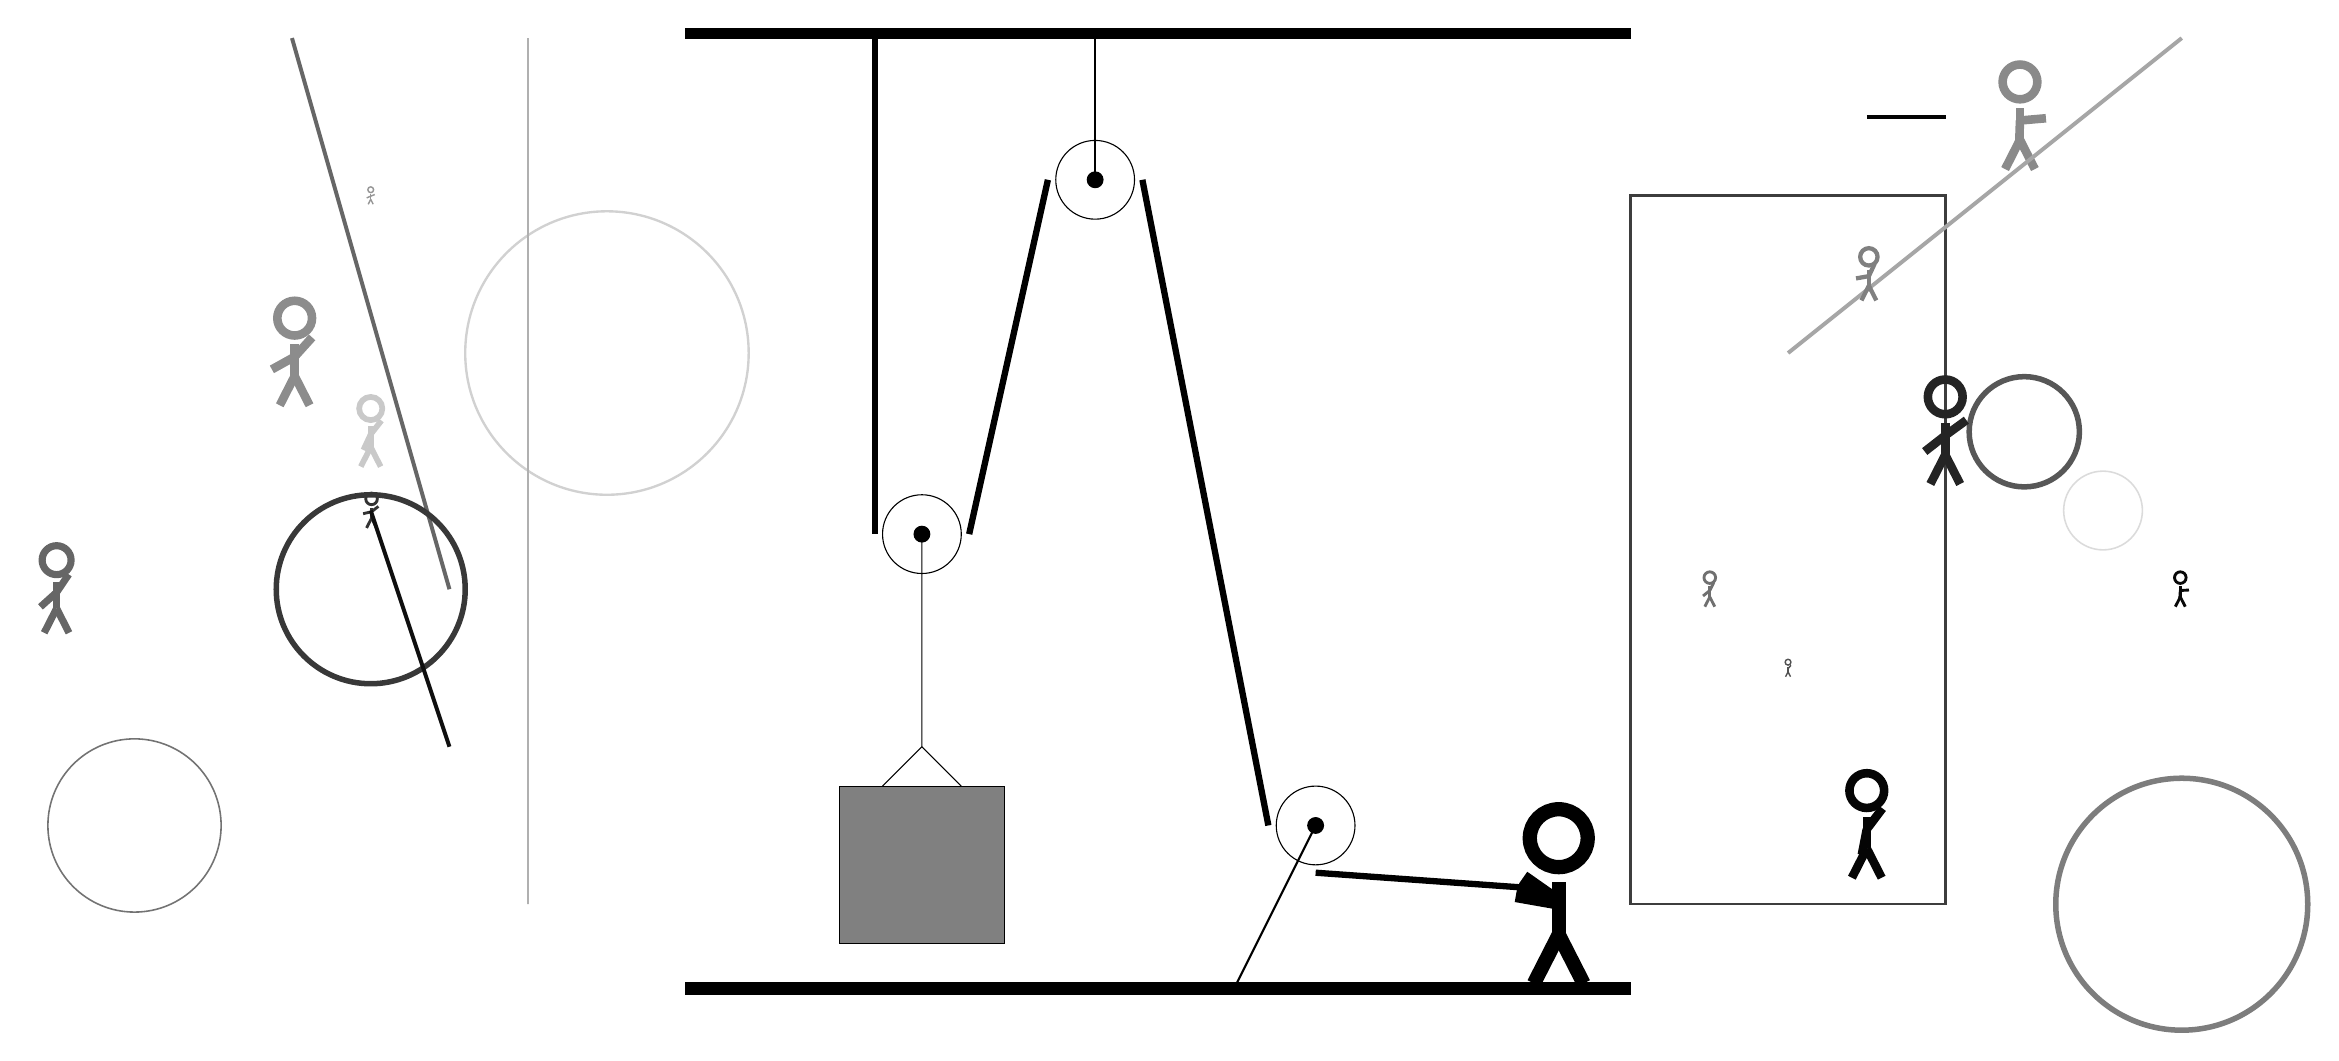
\begin{tikzpicture}
			%%%%% START %%%%%
			
			\draw[fill=black] (-2, 9) rectangle (10, 9.125);
			
			\draw (3.2, 7.2) circle (0.5);
			\draw[fill=black] (3.2, 7.2) circle (0.1);
			\draw[thick] (3.2, 7.2) -- (3.2, 9);
			
			\draw (6, -1) circle (0.5);
			\draw[fill=black] (6, -1) circle (0.1);
			\draw[thick] (6, -1) -- (5, -3);
			
			\draw (1, 2.7) circle (0.5);
			\draw[fill=black] (1, 2.7) circle (0.1);
			
			\node[line width=0.2mm, color=black!80] at (-6, 3) {\Strichmaxerl[2][13][38]};
			
			\draw[line width=0.3mm, color=black!76] (10, 7) rectangle (14, -2);
			\draw [line width=0.7mm, color=black!51](17, -2) circle (1.6);
			\draw[line width=0.5mm, color=black!60](-7, 9) -- (-5, 2);
			\node[line width=0.7mm, color=black!46] at (15, 8) {\Strichmaxerl[6][88][5]};
			\node[line width=0.6mm, color=black!98] at (13, -1) {\Strichmaxerl[6][79][53]};
			
			\draw [line width=0.7mm, color=black!66](15, 4) circle (0.7);
			
			\node[line width=0.4mm, color=black!21] at (-6, 4) {\Strichmaxerl[4][65][52]};
			\node[line width=0.7mm, color=black!56] at (11, 2) {\Strichmaxerl[2][39][63]};
			
			\node[line width=0.5mm, color=black!86] at (14, 4) {\Strichmaxerl[6][38][36]};
			\draw [line width=0.3mm, color=black!18](-3, 5) circle (1.8);
			\draw [line width=0.7mm, color=black!78](-6, 2) circle (1.2);
			\draw[line width=0.3mm, color=black!31] (-4, -2) rectangle (-4, 9);
			
			\node[line width=0.4mm, color=black!60] at (-10, 2) {\Strichmaxerl[5][42][56]};
			\node[line width=0.3mm, color=black!68] at (12, 1) {\Strichmaxerl[1][88][48]};
			\draw[line width=0.5mm, color=black!99](13, 8) -- (14, 8);
			
			\draw[line width=0.5mm, color=black!94](-5, 0) -- (-6, 3);
			\node[line width=0.5mm, color=black!45] at (-7, 5) {\Strichmaxerl[6][29][48]};
			\node[line width=0.2mm, color=black!41] at (-6, 7) {\Strichmaxerl[1][23][22]};
			\draw [line width=0.2mm, color=black!55](-9, -1) circle (1.1);
			\node[line width=0.5mm, color=black!97] at (17, 2) {\Strichmaxerl[2][86][3]};
			
			\draw[line width=0.5mm, color=black!35](12, 5) -- (17, 9);
			\node[line width=0.5mm, color=black!50] at (13, 6) {\Strichmaxerl[3][10][65]};
			\draw [line width=0.2mm, color=black!14](16, 3) circle (0.5);
			
			\draw (1, 2.7) -- (1, 0) -- (0.5, -0.5);
			\draw (1, 0) -- (1.5, -0.5);
			\draw[fill=black!50] (-0.05, -0.5) rectangle (2.05, -2.5);
			
			\draw[line width=0.8mm] (0.4, 9) -- (0.4, 2.7);
			\centerarc[line width=0.8mm](1, 2.7)(180:360:0.6);
			\draw[line width=0.8mm](1.6, 2.7) -- (2.6, 7.2);
			\centerarc[line width=0.8mm](3.2, 7.2)(0:180:0.6);
			\draw[line width=0.8mm](3.8, 7.2) -- (5.4, -1);
			\centerarc[line width=0.8mm](6, -1)(180:270:0.6);
			\draw[line width=0.8mm](6, -1.6) -- (8.8, -1.8);
			
			\node at (9, -1.9) {\Strichmaxerl[10][-35][170]};
			
			\draw[fill=black] (-2, -3) rectangle (10, -3.15);
			
			%%%%% END %%%%%
		\end{tikzpicture}
	\end{figure}	
\end{document}